\begin{comment}
\section{Modi normali della struttura solare}

\begin{frame}[label=noinside]{Modi di oscillazione adiabatici}{Perturbazione dello stato di equilibrio.}

\begin{block}{campi di velocit\'a/effetti non lineari}
Descrivo le oscillazioni come piccole perturbazioni attorno allo stato di equilibrio stazionario (gli effetti non lineari, fra cui lo scambio di energia tra i modi, sono dell'ordine di $\frac{v}{c_s}$ dove v \'e l'ampiezza della velocit\'a dell'oscillazione). 
In generale pu\'o essere presente un campo di velocit\'a $\vec{v}_0$:
\begin{align}
&\vec{v}=\vec{v}_0+\vec{v}'\\
&\TDof{t}=\PDof{t}+(\vec{v}_0\cdot\nabla)
\end{align}
in prima approssimazione prendo $\vec{v}_0=0$ per poi considerare come perturbazioni gli effetti dovuti a campi di velocit\'a in specie rotazione.

\end{block}

\begin{block}{Perturbazione pressione densit\'a}

Indico con $P'(\vec{r},t)$ e $\delta P$ la perturbazione euleriana e lagrangiana della pressione e con $\rho'$, $\Phi'$ e $\vec{g}'$ la perturbazione euleriana della densit\'a , e le perturbazioni euleriane del potenziale gravitazionale e dell'accelerazione di gravit\'a conseguenti  con $\delta\vec{r}=\vec{\xi}$ il vettore spostamento perturbato:
\begin{align}
&P(\vec{r},t)=P_0(\vec{r})+P'(\vec{r},t)\label{eq:pressureperturbation}\\
&\Lvar{P(\vec{r})}=P(\vec{r}+\Lvar{\vec{r}})-P_0(\vec{r})=P'(\vec{r})+\Lvar{\vec{r}}\cdot\nabla P_0\\
&\vec{g}'=-\nabla\Phi',\ \nabla^2\Phi'=4\pi G\rho'\label{eq:gapert}
\end{align}

\end{block}


\end{frame}

\begin{frame}[label=noinside]{Modi di oscillazione adiabatici}{Modi di oscillazione lineari adiabatici.}

\begin{block}{Equazione del moto perturbata}

l'equazione del moto perturbato sostituendo \eqref{eq:pressureperturbation} nell'equazione del moto \eqref{eq:motion} considerando solo i termini lineari nella perturbazione:
\begin{equation}
\rho_0\TDof{t}\vec{v}=\rho_0\PtwoDy{t}{\Lvar{\vec{r}}}=-\nabla P'+\rho_0\vec{g}'+\rho'\vec{g}_0\label{eq:emper}
\end{equation}

\end{block}

\end{frame}

\begin{frame}[label=noinside]{Modi di oscillazione adiabatici}{Equazione di continuit\'a perturbata}

\begin{block}{Equazione di continuit\'a perturbata}

Analogamente per l'equazione di continuit\'a ottengo
\begin{equation}
\rho'+\div{(\rho_0\Lvar{\vec{r}})}=0\label{eq:contper}
\end{equation}

\end{block}

\end{frame}

\begin{frame}[label=noinside]{Modi di oscillazione adiabatici}{Condizione di adiabaticit\'a}


  \begin{overlayarea}{\textwidth}{1cm}
   \only<1>{
   energia interna per unit\'a di massa
\begin{equation}
\TDy{t}{q}=\TDy{t}{u}+P\TDof{t}(\frac{1}{\rho})\label{eq:prima}
\end{equation}

\begin{equation}
\TDy{t}{T}-\frac{\Gamma_2-1}{\Gamma_2}\frac{T}{P}\TDy{t}{P}=\frac{1}{c_P}(\epsilon-\frac{1}{\rho}\scap{\nabla}{F})
\end{equation}
il termine a destra \'e trascurabile:
\begin{equation}
\TDy{t}{q}=0
\end{equation}
   }
   \only<2>{
   Il moto di una elemento di fluido \'e descritto dalla relazione adiabatica
\begin{equation}
\TDy{t}{P}=\frac{\Gamma_1P}{\rho}\TDy{t}{\rho}
\end{equation}
}
   \only<3>{
  
  La condizione di perturbazione adiabatica linearizzata \'e
\begin{align}
&\PDy{t}{\Lvar{P}}-\frac{\Gamma_{1,0}P_0}{\rho_0}\PDy{t}{\Lvar{\rho}}=0\\
&P'+\Lvar{\vec{\xi}}\cdot\nabla P_0=\frac{\Gamma_{1,0}P_0}{\rho}(\rho'+\Lvar{\vec{\xi}}\cdot\nabla\rho_0)\label{eq:adper}
\end{align}

   }
  \end{overlayarea}


\end{frame}


\begin{figure}[!ht]

\subfigure[Distribuzione dei modi con $l\leq300$ nel diagramma $\nu-l$ determinata usando i primi 144 giorni di osservazione di MDI. Da \cite{chr02helioseismology}.]{
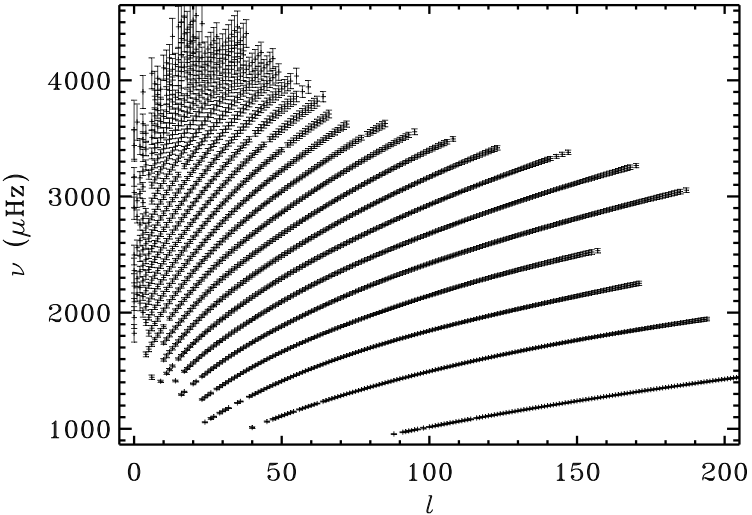
\includegraphics[keepaspectratio,width=0.45\textwidth]{midlmodes}}
\label{fig:midlmodes}
~
\subfigure[Modi adiabatici calcolati sulla base di un modello solare. Da \cite{chr02helioseismology}.]{
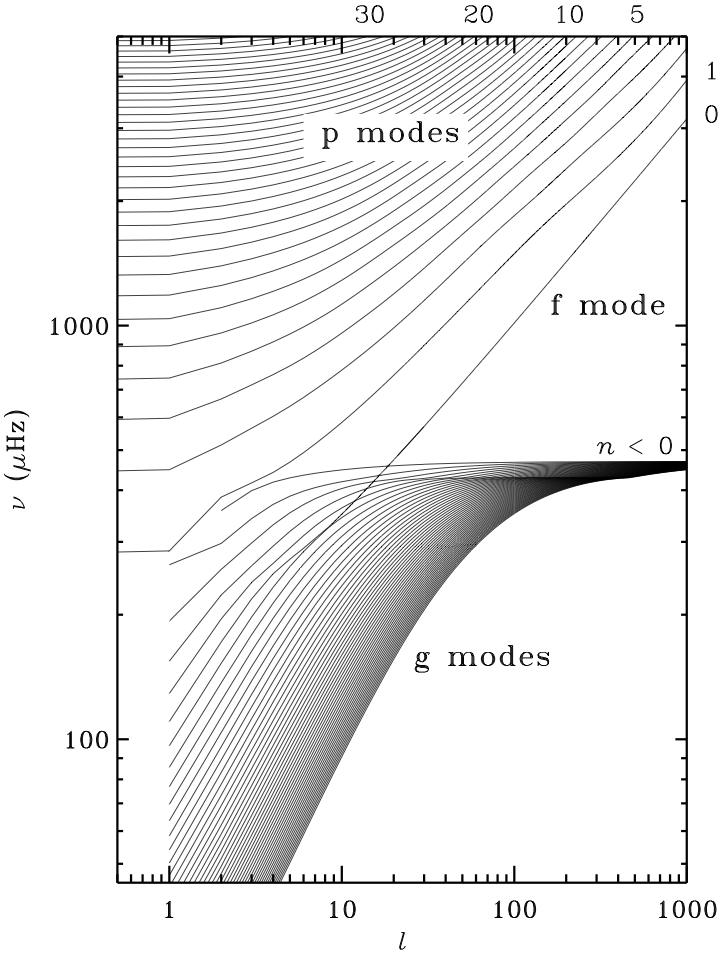
\includegraphics[keepaspectratio,width=0.6\textwidth]{nrmodesLAWE}\label{fig:nrmodesLAWE}}

\end{figure}
\end{comment}

%%% SOS

\section{Modi normali della struttura solare}

\begin{frame}{Oscillazioni dei 5 minuti}

\begin{block}{Comportamento periodico dell'atmosfera solare con grande coerenza spaziale e temporale}

\citet{lei62velocity}: la superficie solare ha scale spazio-temporali privilegiate - comportamento periodico nell'atmosfera a tutte le altezze, $\Pi\approx\SI{300}{\second}$ secondi e $\lambda_h\approx\si{\mega\meter}$.

\end{block}

\begin{block}{Modi normali - onde gravo-acustiche in cavit\'a risonanti di varia profondit\'a}

Modi p: modi acustici - $\Pi\approx\SI{5}{\minute}$.

Modi g: onde di gravit\'a.

Modi f: onde di superficie.

Rumore solare a basse frequenze e ai processi di eccitazione dei modi che trasferiscono la massima energia ai modi di tale periodo.

\citet{ulrich70five} e \citet*{stein71five}: relazione di dispersione per onde acustiche evidenzia la presenza di cavit\'a risonanti all'interno del Sole.
% La variazione delle propriet\'a del gas delimita le regioni di propagazione a diverse profondit\'a a seconda delle caratteristiche trasversali del moto: $\lambda_h=\frac{2\pi}{k_h}\approx\frac{2\pi R}{\sqrt{l(l+1)}}$

\end{block}

\end{frame}

\subsection{Perturbazione adiabatiche.}

\begin{frame}{Equazioni di conservazione perturbate}

%con $\vec{v}'$ perturbazione euleriana della velocit\'a. La variazione di una grandezza euleriana nel riferimento solidale con l'elemento di fluido si esprime tramite

\begin{block}{Perturbazioni densit\'a e pressione}

\begin{align}
&\vec{v}=\vec{v}_0+\vec{v}'\ \TDof{t}=\PDof{t}+(\vec{v}_0\cdot\nabla)\\
&P(\vec{r},t)=P_0(\vec{r})+P'(\vec{r},t)\label{eq:pressureperturbation}\\
&\Lvar{P(\vec{r})}=P(\vec{r}+\Lvar{\vec{r}})-P_0(\vec{r})=P'(\vec{r})+\Lvar{\vec{r}}\cdot\nabla P_0\\
&\vec{g}'=-\nabla\Phi',\ \nabla^2\Phi'=4\pi G\rho'\label{eq:gapert}
\end{align}

\end{block}

%Ricavo l'equazione del moto perturbato sostituendo \eqref{eq:pressureperturbation} nell'equazione del moto \eqref{eq:motion} considerando solo i termini lineari nella perturbazione:
\begin{block}{Equazione di continuit\'a e del moto perturbate}

\begin{align}
&\rho_0\TDof{t}\vec{v}=\rho_0\PtwoDy{t}{\vec{\xi}}=-\nabla P'+\rho_0\vec{g}'+\rho'\vec{g}_0\label{eq:emper}\\
&\rho'+\div{(\rho_0\Lvar{\vec{r}})}=0\label{eq:contper}
\end{align}

\end{block}

\end{frame}

\begin{frame}{Perturbazione adiabatica}

%L'equazione di conservazione dell'energia interna \eqref{eq:primatemp}, esplicitando il bilancio di calore \eqref{eq:heatgl}, \'e
\begin{equation}
\TDy{t}{T}-\frac{\Gamma_2-1}{\Gamma_2}\frac{T}{P}\TDy{t}{P}=\frac{1}{c_P}(\epsilon-\frac{1}{\rho}\scap{\nabla}{F})
\end{equation}
%Mostro schematicamente che il termine a destra \'e trascurabile su tempi del periodo delle oscillazioni solari.

Entrambi i tempi scala per scambio di calore sono molto maggiori del periodo delle oscillazioni quindi su un periodo i termini dovuti allo scambio di calore sono trascurabili; l'approssimazione adiabatica non \'e pi\'u valida vicino alla superficie solare dove i tempi per lo scambio di calore sono pi\'u brevi.
%Il moto di una elemento di fluido \'e descritto dalla relazione adiabatica linearizzata
%\begin{equation}
%\TDy{t}{P}=\frac{\Gamma_1P}{\rho}\TDy{t}{\rho}
%\end{equation}
La condizione di perturbazione adiabatica linearizzata \'e:
\begin{align}
&\PDy{t}{\Lvar{P}}-\frac{\Gamma_{1,0}P_0}{\rho_0}\PDy{t}{\Lvar{\rho}}=0\\
&P'+\vec{\xi}\cdot\nabla P_0=\frac{\Gamma_{1,0}P_0}{\rho}(\rho'+\vec{\xi}\cdot\nabla\rho_0)\label{eq:adper}
\end{align}

\end{frame}

\begin{frame}{Oscillazioni di equilibrio a simmetria sferica}

%Cerco una soluzione della forma di un'onda stazionaria: esprimo la dipendenza temporale tramite $\exp{i\omega t}$ e angolare tramite le funzioni armoniche sferiche $Y_{lm}(\theta,\phi)$ con:
\begin{align}
&Y_{lm}(\theta,\phi)=(-)^mc_{lm}P_l^m(\cos{\theta})\exp{im\phi}\\
%&L^2Y_l^m=-\frac{1}{\sin{\theta}}\PDof{\theta}(\sin{\theta}\PDy{\theta}{Y_l^m})+\frac{1}{\sin^2{\theta}}\PtwoDy{\phi}{Y_l^m}=-r^2\nabla_h^2Y_l^m=l(l+1)Y_l^m\label{eq:SHperturb}
\end{align}
Oscillazioni di una struttura di equilibrio a simmetria sferica
\begin{equation}
(\rho',P',\Phi')=\exp{i\omega t}[\rho'(r),P'(r),\Phi'(r)]Y_l^m
\end{equation}

%Dall'equazione del moto \eqref{eq:emper}, poich\'e le deviazioni dalla simmetria sferica sono in prima approssimazione trascurabili, \'e evidente che:
\begin{equation}
%&\omega^2\vec{\xi}=\nabla a+\frac{N^2c^2}{g}b\frac{\vec{r}}{r}\\
\hat{r}\cdot(\rot{\vec{\xi}})=0\ \Rightarrow\ \PDof{\theta}(\sin{\theta}\xi_{\phi})-\PDy{\phi}{\xi_{\theta}}=0
\end{equation}
ed \'e quindi possibile ricavare la componente tangenziale della perturbazione da una funzione scalare:
\begin{equation}
\vec{\xi}=\exp{i\omega t}(\xi_r(r),\xi_h(r)\PDof{\theta},\frac{\xi_h(r)}{\sin{\theta}}\PDof{\phi})Y_l^m(\theta,\phi)
\end{equation}
dove ho scomposto il vettore spostamento perturbato in componente radiale $\xi_r(r)$ e tangenziale $\xi_h(r)$.

\end{frame}

\begin{frame}{Modi normali adiabatici}

%Ricavo la componente $\xi_h(r)$ applicando la parte tangenziale della divergenza all'equazione del moto:
\begin{equation}
\xi_h(r)=\frac{L}{r\omega^2}(\frac{P'(r)}{\rho_0}+\Phi'(r))
\end{equation}
%infine $\xi_r(r)$, $P'(r)$ e $\Phi'(r)$ sono determinati da
\begin{subequations}\label{eigenomega}
\begin{align}
&\frac{1}{r^2}\TDof{r}(r^2\xi_r)-\frac{\xi_rg}{c^2}+\frac{1}{\rho_0}(\frac{1}{c^2}-\frac{l(l+1)}{r^2\omega^2})P'-\frac{l(l+1)}{r^2\omega^2}\Phi'=0\\
&\frac{1}{\rho_0}(\TDof{r}+\frac{g}{c^2})P'-(\omega^2-N^2)\xi_r+\TDy{r}{\Phi'}=0\\
&\frac{1}{r^2}\TDof{r}(r^2\TDy{r}{\Phi'})-\frac{l(l+1)}{r^2}\Phi'-\frac{4\pi G\rho_0}{g}N^2\xi_r-\frac{4\pi G}{c^2}P'=0
\end{align}
\end{subequations}
%con $g=-\frac{1}{\rho_0}\TDy{r}{P_0}$.

Condizioni al contorno: sono necessarie 4 condizioni.
\begin{itemize}
\item Due condizioni per $r=0$ selezionano le soluzioni regolari:
\begin{equation}
P'=0,\ \Phi'=0
\end{equation}
%Vicino a zero risulta un andamento asintotico
%\begin{equation}
%(l\neq0):\ \xi_r\propto r\expy{l-1};\ (l=0):\ \xi_r\propto r;P',\ \Phi'\propto r^l
%\end{equation}

\item Alla superficie solare richiediamo la continuit\'a di $\Lvar{\nabla\Phi}$ e che non si abbia propagazione verso l'esterno.
%All'esterno della stella ho $\rho'=0$ quindi scelgo la soluzione nulla a infinito dell'equazione di Poisson $\Phi'=Ar\expy{-l-1}$:
%\begin{equation}
%\TDy{r}{\Phi'}+\frac{l+1}{r}\Phi'=0,\ r=\rsun{}    
%\end{equation}
%La condizione di non propagazione oltre la fotosfera dipende dalla descrizione dell'atmosfera solare. Nella versione pi\'u semplice impongo che la variazione di pressione sia zero alla superficie perturbata della stella
%\begin{align}
%&\Lvar{P}=P'+\xi_r\TDy{r}{P}=0
%\end{align}
\end{itemize}

\end{frame}

\begin{frame}{Diagramma $\nu-l$ per i modi adiabatici}

Il sistema di equazione \eqref{eigenomega} ha soluzione per $\omega_{nlm}$ discrete, m non compare esplicitamente quindi sono $2l+1$ degeneri.

\begin{figure}[!ht]
\subfigure[I picchi della densit\'a spettrale si dispongono su creste nel diagramma $\nu-l$.]{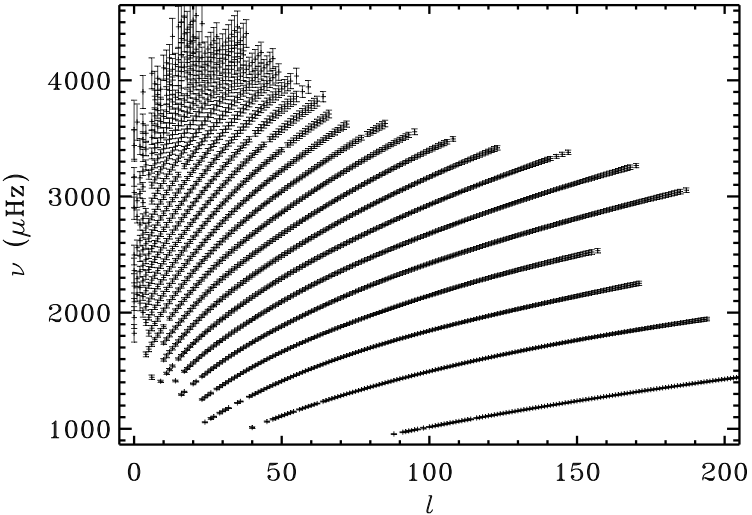
\includegraphics[keepaspectratio,width=0.4\textwidth]{midlmodes}}
\label{fig:midlmodes}
~
\subfigure[Modi adiabatici calcolati sulla base di un modello solare. .]{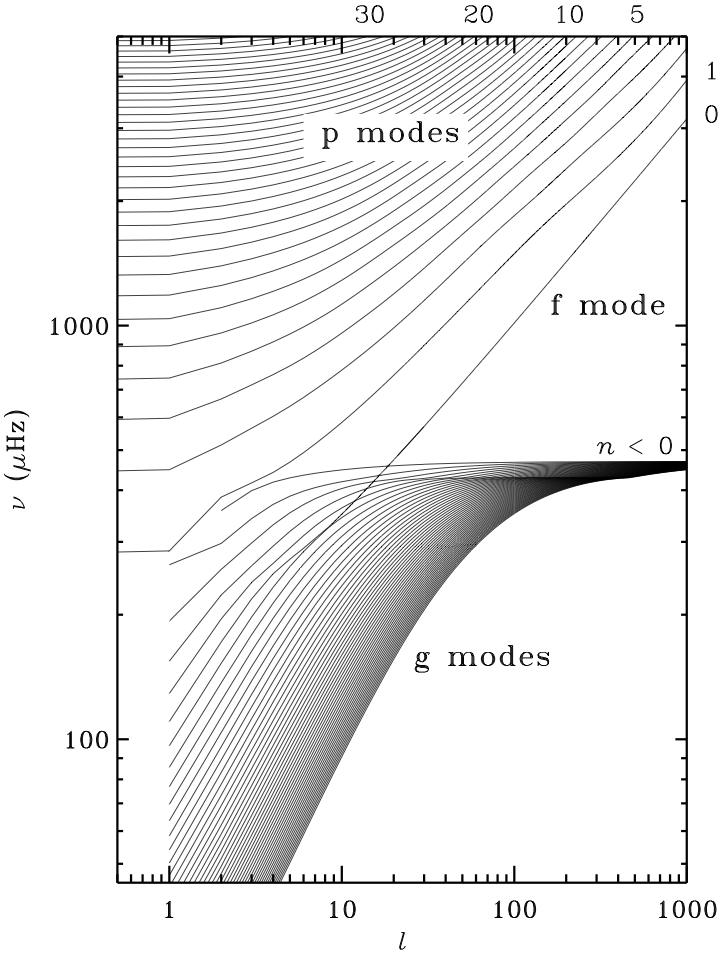
\includegraphics[keepaspectratio,width=0.4\textwidth]{nrmodesLAWE}}
\label{fig:nrmodesLAWE}

\end{figure}

\end{frame}

\subsection{Energia dei modi-effetti di superficie}

\begin{frame}{Energia dei modi}

Indico con $\exv{E_{kin}^{nl}}$ la media temporale dell'energia cinetica del modo
\begin{equation}
E_{kin}^{nl}=\frac{1}{2}\int_V|\vec{v}|^2\rho_0\,dV=\frac{\omega^2}{2}\int_V|\vec{\xi}|^2\rho_0\,dV
\end{equation}
cio\'e
\begin{equation}
\exv{E_{kin}^{nl}}=\frac{1}{\Pi}\int_0^{\Pi}E_{kin}^{nl}=\frac{1}{2}I_{nl}\exv{\dvec{\xi}_{nl}(R)}^2
\end{equation}
dove $\exv{\dvec{\xi}_{nl}(R)}$ indica la velocit\'a quadratica media superficiale e ho definito l'inerzia normalizzata:
\begin{equation}\label{eq:normalizedinertia}
I_{nl}=\frac{1}{M\exv{\vec{\xi}(R)\vec{\xi}^*(R)}}\int_V\,d^3x\rho_0\vec{\xi}\vec{\xi}^*
\end{equation}

\end{frame}

\begin{frame}{Accordo frequenze osservate vs calcolate tramite MSS}

\begin{columns}

\begin{column}{0.45\textwidth}
\begin{figure}[!ht]
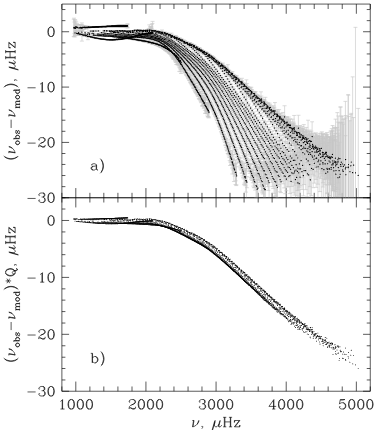
\includegraphics[keepaspectratio,width=0.9\textwidth]{domega}
%\subfigure[Differenza di fase per il segnale Doppler delle righe $(5930)$ Fe I, pi\'u profonda, e $(5896)$ Na I, pi\'u alta nell'atmosfera. Da \cite{staiger1987observations}.]{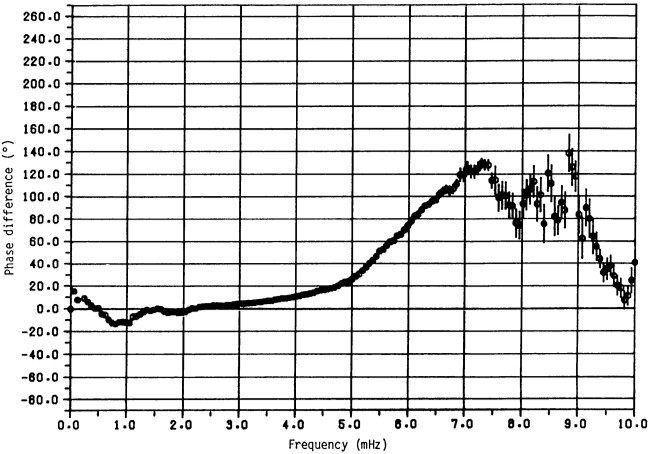
\includegraphics[keepaspectratio,width=0.4\textwidth]{phasepropagation}}
%\label{fig:phasedifference}
%~
%\subfigure[In alto: differenze tra frequenze dei modi teoriche e osservate. In basso: differenze moltiplicata per $Q_{nl}$.]{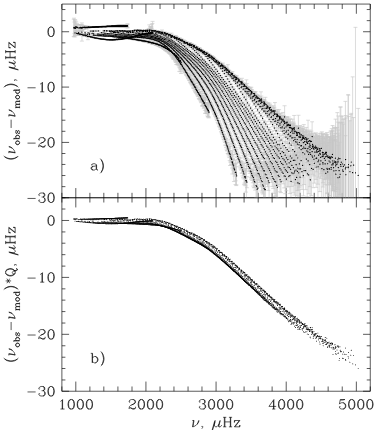
\includegraphics[keepaspectratio,width=0.4\textwidth]{domega}}
%\label{fig:nFreqdiff}
\end{figure}
\end{column}

\begin{column}{0.45\textwidth}
\captionof{figure}{In alto: differenze tra frequenze dei modi teoriche e osservate. In basso: differenze moltiplicata per $Q_{nl}$.}
\end{column}

\end{columns}

Gli effetti dovuti alla non corretta descrizione fisica dei modi vicino alla superficie, $r>0.95\rsun{}$ sono maggiori per i modi di l elevato perch\'e confinati in gusci meno profondi al crescere di l e crescono con $\nu_{nl}$ perch\'e la riflessione avviene pi\'u in alto.

%Nella figura (\subref{fig:nrmodesLAWE}) sono mostrate le frequenze dei modi soluzioni del sistema \eqref{eigenomega} calcolati usando le grandezze di equilibrio di un modello solare, in (\subref{fig:midlmodes}) le frequenze misurate e in \subref{fig:nFreqdiff} le differenze tra frequenze predette e osservate.
% Introduco il rapporto d'inerzia:
%\begin{align}
%&\frac{V_{nl}}{V_0(\nu_{nl})}=(Q_{nl})\expy{-\midfrac{1}{2}}\intxt{dove ho introdotto l'inerzia e il rapporto d'inerzia $Q_{nl}$}
%&Q_{nl}=\frac{I_{nl}}{I^0_{nl}}\label{eq:surfaceeffects}
%\end{align}
%$Q_{nl}=1$ per $l=0$ e diminuisce al crescere di $l$; l'ampiezza superficiale relativa al modo radiale estrapolato a frequenza $\nu_{nl}$, $\frac{A_{nl}(\nu_{nl})}{A_{nl}^0(\nu_{nl})}\propto(Q_{nl})\expy{-\midfrac{1}{2}}$, cresce con l.

%Il comportamento all'aumentare della frequenza mostrato in \subref{fig:nFreqdiff} \'e dovuto al fatto che per frequenze maggiori la regione in cui si ha riflessione interna \'e pi\'u in alto dove l'approssimazione adiabatica \'e meno valida; la figura \subref{fig:phasedifference} mostra la propagazione di fase ad alte frequenze dovuta ad effetti dissipativi.

\end{frame}

\subsection{Principio variazionale}    %Vedi pg 110 dalsnote.

\begin{frame}{Variazioni nel modello provocano variazioni nelle frequenze dei modi}

Equazione del moto perturbata:
\begin{align*}\label{eq:EOMrhoc}%Unno89
&-\omega^2\rho_0\xi=\nabla(c_s^2\rho\scap{\nabla}{\xi}+\nabla P\cdot\vec{\xi})-\vec{g}_0\nabla\cdot(\rho_0\vec{\xi})\\
&-G\rho_0\nabla(\int_V\frac{\nabla\cdot(\rho_0\vec{\xi})\,d^3r'}{|\vec{r}-\vec{r}'|})
\end{align*}

\citet{Cha64Variational} ha dimostrato che questo costituisce un problema agli autovalori hermitiano per condizioni ai bordi di pressione e densit\'a nulle%quindi $\omega^2$ \'e reale e autofunzioni di frequenza caratteristica diversa sono ortogonali:
%\begin{equation}
%\int\vec{\xi}_i*\vec{\xi}_j\rho\,d^3x=0
%\end{equation}

Relazione tra variazioni nell'operatore lineare $L(\vec{\xi})=-\omega^2\vec{\xi}$ e differenze nelle frequenze caratteristiche:
%\begin{equation}
%(L+\Lvar{L})(\xi+\Lvar{\xi})=-(\omega+\Lvar{\omega})^2(\xi+\Lvar{\xi})\label{eq:EMvar}
%\end{equation}
quindi considerando i termini lineari nelle variazioni e dato che le frequenze caratteristiche sono stazionarie per variazioni di $\xi$ si ha la relazione:
\begin{equation}\label{eq:variational}
\frac{\Lvar{\omega}}{\omega}=-\frac{\int_V\rho\vec{\xi}\Lvar{L}\vec{\xi}\,d^3x}{2\omega^2\int_V\rho\scap{\xi}{\xi}d^3x}
\end{equation}

\end{frame}

\subsection{Variazioni struttura idrostatica e variazioni nell'equazione di stato e nella  composizione}

\begin{frame}{Variazioni struttura idrostatica}

La forma della perturbazione $\delta L$ permette di scrivere%in \eqref{eq:EOMrhoc} introducendo piccole variazioni nel profilo di $\rho$ e $c_s$:
%\begin{equation}
%\Lvar{L}\vec{\xi}=\nabla(\Lvar{c_s^2}\nabla\cdot\vec{\xi}+\Lvar{\vec{g}}\cdot\vec{
%\xi})+\nabla(\frac{\Lvar{\rho}}{\rho_0})c^2\nabla\cdot\vec{\xi}+\frac{1}
%{\rho_0}\nabla\rho_0\Lvar{c_s^2}\nabla\vec{\xi}+\Lvar{\vec{g}}\nabla\cdot\vec{\xi}-
%G\nabla\int_V\frac{\nabla\cdot(\Lvar{\rho}\xi)}{|\vec{x}-
%\vec{x}'|}\,d^3x'\label{eq:eqmotvar}
%\end{equation}
%con
%\begin{equation}
%\Lvar{g}(r)=\frac{4\pi G}{r^2}\int_0^r\Lvar{\rho}(s)s^2\,ds
%\end{equation}
%\'E quindi possibile esprimere le differenze nelle frequenze dei modi nella forma
\begin{equation}\label{eq:hydroefdiff}
\frac{\delta\omega_{nl}}{\omega_{nl}}=\int_0^R[K^{nl}_{c^2,\rho}(r)\frac{\delta_rc^2}{c^2}(r)+K^{nl}_{\rho,c^2}(r)\frac{\delta_r\rho}{\rho}(r)]\,dr+I_{nl}\expy{-1}F_{Surf}
\end{equation}

I kernel $K_Q^j$ dipendono dalle autofunzioni del modello solare, il termine $I_{nl}\expy{-1}F_{Surf}(\omega_{nl})$ tiene conto degli effetti superficiali.

\begin{equation}
\Lvar{P}=\int_r^R(g\Lvar{\rho}+\rho\Lvar{g})\,dr\label{eq:pressurecorrho}
\end{equation}

\end{frame}

\begin{frame}{Variazioni equazione di stato e composizione}

Dipendenza di $\Gamma_1(P,\rho,X_i)$ dalla composizioneriscrivendo \eqref{eq:hydroefdiff} nella forma:
\begin{align*}
&\frac{\delta\omega_{nl}}{\omega_{nl}}=\int_0^R[K^{nl}_{\Gamma_1,\rho}(r)\frac{\delta_r\Gamma_1}{\Gamma_1}(r)+K^{nl}_{\rho,\Gamma_1}(r)\frac{\delta_r\rho}{\rho}(r)]\,dr\\
&+I_{nl}\expy{-1}F_{Surf}(\omega_{nl})\\%\label{eq:invdGammadrho}\\
&=\int_0^R[K^{nl}_{u,Y}(r)\frac{\delta_ru}{u}(r)\,dr+K^{nl}_{Y,u}(r)\delta_rY\,dr+K^{nl}_{c^2,\rho}(r)(\frac{\delta\Gamma_1}{\Gamma_1})_{int}]\,dr\\
&+I_{nl}\expy{-1}F_{Surf}(\omega_{nl})%\label{eq:diffthermo}
\end{align*}
dove $(\delta\Gamma_1)_{int}$ \'e la variazione all'equazione di stato a $(P,\rho,Y)$ fissati.

La determinazione dell'abbondanza di elio nella regione convettiva \'e dovuta principalmente alla deviazione da $\Gamma_1=\frac{5}{3}$ nella regione di seconda ionizzazione dell'elio.

\end{frame}


\section{Campo di velocit\'a solare}

\subsection{Analisi fenomeni stazionari stocastici}

\begin{frame}{Misura velocit\'a Doppler}

%I fenomeni periodici sulla superficie solare sono osservabili tramite tecniche fotometriche o spettroscopiche, tramite effetto doppler: una parte basilare dell'informazione contenuta nei modi di oscillazione \'e ricavata analizzando  lo spostamento doppler delle righe di assorbimento dei metalli presenti negli strati visibili pi\'u esterni del sole.

L'ampiezza della velocit\'a di oscillazione per il singolo modo \'e  al pi\'u \SI{15}{\cm\per\second}% quindi l'effetto doppler causa uno shift, al massimo, di $\frac{\Delta\lambda}{\lambda}\approx\num{e-10}$. 
Le misure Doppler su luce integrata sull'intero disco solare sono effettuate tramite uno spettroscopio a scattering risonante, in cui lo splitting  Zeeman dovuto a un campo magnetico esterno applicato a vapori di $Na/K$ permette la trasmissione  in due bande molto strette simmetriche rispetto alla linea spettrale di cui si vuole misurare lo shift: la velocit\'a Doppler \'e proporzionale alla differenza di intesit\'a osservata nelle due bande. Il tacometro di Fourier \'e uno degli strumenti pi\'u utilizzati per misure Doppler  con risoluzione spaziale.

%Il fattore $\sin{\theta}\cos{\phi}$ deriva dalla proiezione della velocit\'a radiale sulla linea di vista: i modi con periodo attorno ai 5 minuti di grado l non elevato causano uno spostamento quasi totalmente radiale:
%\begin{align}
%&\frac{\delta h|_{rms}}{\delta r|_{rms}}=\frac{\sqrt{l(l+1)}}{\sigma^2}\\
%&\sigma^2=\frac{\rsun{}}{G\msun{}}\omega^2\approx1000
%\end{align}
%Per isolare il contributo di una singola $Y_{l_0m_0}$ considero
\begin{align*}%\label{eq:dopplerTS}
&V_D(\theta,\phi,t)=\sin{\theta}\cos{\phi}\sum_{n,l,m}A_{nlm}c_{lm}P_l^m(\cos{\theta})\cos{(m\phi-\omega_{nlm}t-\beta_{nlm})}\\
&V_{l_0m_0}(t)=\int_AV_D(\theta,\phi,t)W_{l_0m_0}(\theta,\phi)\,dA\\
&=\sum_{n,l,m}S_{l_0m_0,lm}A_{nlm}(t)\cos{(\omega_{nlm}t+\beta_{nlm,L_0m_0})}
\end{align*}
%e ho integrato sul disco solare con $W_{l_0m_0}\approx Y_{l_0m_0}$. $S_{l_0m_0,lm}$ \'e la funzione di risposta che non \'e esattamente $\propto\delta_{ll_0}\delta_{mm_0}$ poich\'e le armoniche sferiche sono ortogonali sull'intera sfera ma contiene contributi da valori di $(l,m)$ vicini.

\end{frame}

\begin{comment}
\begin{align}
&\delta r|_{rms}=\exv{\vec{\xi}\cdot\hat{r}}=\frac{1}{2}|\tilde{xi}_r|^2\\
&=\frac{1}{\Pi}\int_0^{\pi}\,dt\frac{1}{4\pi}\oint\Re{\tilde{\xi}_rY_{l,m}(\theta,\phi)\exp{-i\omega t}}^2\,d\omega\\
&\delta h_{rms}^2=\exv{|\vec{\xi}_h|^2}=\frac{1}{2}l(l+1)|\tilde{\xi}_h(r)|^2\\
&\frac{\delta h|_{rms}}{\delta r|_{rms}}=\frac{\sqrt{l(l+1)}}{\sigma}
\end{align}
\end{comment}

\begin{frame}{Fenomeni stazionari stocastici}
Considero la trasformata di Fourier del segnale Doppler per tempo di osservazione $T$

\begin{columns}

\begin{column}{0.5\textwidth}

\begin{equation*}
V_{l_0m_0}(\nu)=\int_{-\midfrac{T}{2}}^{\midfrac{T}{2}}V_{l_0m_0}(t)\exp{i2\pi\nu t}\,dt
\end{equation*}

\end{column}

\begin{column}{0.5\textwidth}
\begin{align*}
&\Delta\omega=\frac{2\pi}{T}\leq\omega\leq\frac{\pi}{\Delta t}\\
&\Delta k_i=\frac{2\pi}{L_i}\leq k_i\leq\frac{\pi}{\Delta x_i}
\end{align*}
\end{column}

\end{columns}

Considero la trasformata di Fourier di un processo stocastico $x(t)$ campionato per un tempo T $X_T(\nu)$:
\begin{align*}
%&X_T(\nu)=\int_{-\frac{T}{2}}^{\frac{T}{2}}x(t)\exp{i2\pi\nu t}\\
%\intxt{la cui densit\'a spettrale di potenza (DSP) \'e}
&P_T(\nu)=\frac{1}{T}|X_T(\nu)|^2%\label{eq:powerspectraldensity}
%&S_T(\nu)=\frac{1}{T}\int_{-T/2}^{T/2}\int_{-T/2}^{T/2}x(t)x(t')\exp{i2\pi\nu t}\exp{i2\pi\nu t}\,dt\,dt'\\
=\int_{-T/2}^{T/2}\left[\frac{1}{T}\int_{-T/2}^{T/2}x(t')x(t'+\tau)\,dt'\right]\exp{i2\pi\nu \tau}\,d\tau\\
&P_T(\nu)=\int_{-T/2}^{T/2}C_T(\tau)\exp{i2\pi\nu\tau}\,d\tau\\
&C(\tau)=E(x(t)x(t+\tau))=\lim_{T\to\infty}{C_T(\tau)}
\end{align*}



%Un segnale di durata T permette una risoluzione $\Delta\omega=\frac{2\pi}{T}$ mentre il limite superiore delle frequenze osservate \'e dato dalla frequenza di Nyquist $\omega_{Ny}=\frac{\pi}{\Delta t}$ con $\Delta t$ risoluzione temporale; nel caso le dimensioni lineari $L_i$ della regione osservata siano piccole da poter trascurare la curvatura si hanno analoghe relazioni per le variabili spaziali cartesiane e vettore d'onda associato:
%I modi normali sono identificati tramite la distribuzione spaziale delle oscillazioni in superficie, cio\'e tramite $(l,m)$ o, approssimando localmente l'oscillazione con un onda piana, tramite $k_h$, con
%\begin{equation}
%\vec{k}=k_r\hat{r}+\vec{k}_h,\ k_h^2=\frac{l(l+1)}{r^2}
%\end{equation}
%e dalla distribuzione delle frequenze, che identifica l'ordine n ovvero il numero di zeri radiali della velocit\'a perturbata.


\end{frame}

\begin{frame}{Densit\'a spettrale per osservazioni sull'intero disco}

\begin{figure}[!ht]
\centering
\subfigure[Densit\'a spettrale modi p di basso grado angolare. Da \cite{chr02helioseismology}.]{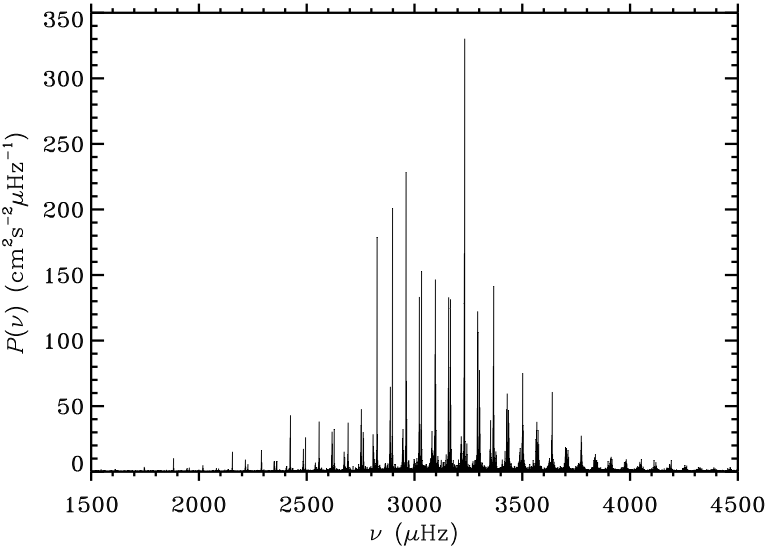
\includegraphics[keepaspectratio,width=0.5\textwidth]{lowlmodes}}
%\caption{Densit\'a spettrale modi p di basso grado angolare. Da \cite{chr02helioseismology}.}\label{fig:lowlmodes}
%\begin{figure}[!ht]
%\centering
\subfigure[Densit\'a spettrale di oscillatore smorzato di frequenza naturale $\midfrac{\omega_{nl}}{2\pi}$ con forzante stocastica. $P_f$ \'e la DSP della forzante. $P=P_fP_L$. Da \cite{houdek2006stochastic}.]{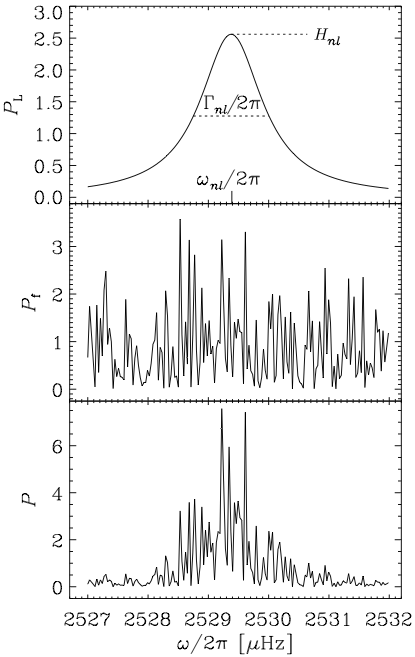
\includegraphics[keepaspectratio,width=0.35\textwidth]{Powerspectraldensity}}
%\caption{Densit\'a spettrale di oscillatore smorzato di frequenza naturale $\midfrac{\omega_{nl}}{2\pi}$ con forzante stocastica. $P_f$ \'e la DSP della forzante. $P=P_fP_L$. Da \cite{houdek2006stochastic}.}\label{fig:Powerspectraldensity}
%\end{figure}
\end{figure}

\end{frame}

\begin{frame}{Forma del picco della densit\'a spettrale di potenza}

%\begin{columns}
%\begin{column}{0.4\textwidth}

Il valore di aspettazione della densit\'a spettrale per un tempo di osservazione tendente a infinito \'e:
\begin{align}
&P_x(\nu)=\lim_{T\to\infty}{E[P_T(\nu)]}=\int_{-\infty}^{-\infty}C(\tau)\exp{2\pi i\nu\tau}\,d\tau\\
%\intxt{da cui si ha il teorema di Wiener-Khinchin}
&C(\tau)=\int_{-\infty}^{-\infty}P_x(\nu)\exp{-2\pi i\nu\tau}\,d\nu\\
%\intxt{che per $\tau=0$ da l'identit\'a di Parseval:}
&C(0)=\int_{-\infty}^{-\infty}P_x(\nu)\,d\nu=E(x^2)
\end{align}

Il segnale solare osservato \'e sovrapposizione di un segnale armonico e del rumore: la densit\'a spettrale si scrive
\begin{equation}
P_x(\nu)=\sum_i\frac{AB_i\midfrac{\Gamma^2}{4}}{(\nu-\nu_0-\Delta\nu_i)^2+\midfrac{\Gamma^2}{4}}+P_n(\nu)
\end{equation}
dove $A$ \'e l'altezza del picco $\Gamma$ la larghezza a met\'a altezza, i termini $\Delta\nu_i$ e $B_i$ descrivono i lobi parassiti; il secondo termine descrive il rumore solare e strumentale.

\end{frame}

%\end{column}

%\begin{column}{0.6\textwidth}

\begin{frame}{Modello dell'ampiezza superficiale delle oscillazioni}

\begin{columns}

\begin{column}{0.4\textwidth}

\begin{figure}[!ht]
\centering
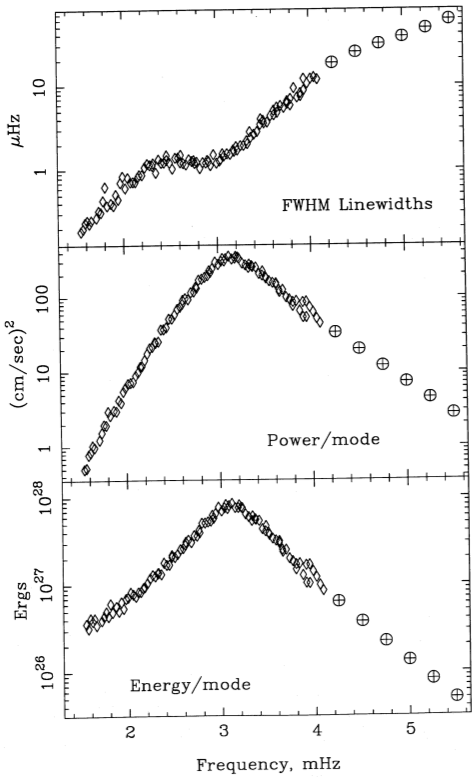
\includegraphics[keepaspectratio,width=0.85\textwidth]{modespheomenology}
\caption{Risultati osservativi per $\Gamma$, $\exv{V^2}$ e $E_{nl}$ per modi con $l\approx20$. Da \cite{libbrecht1988solar}.}\label{fig:Powerspectraldensity}
\end{figure}

\end{column}

\begin{column}{0.6\textwidth}

%Il profilo lorentziano della densit\'a spettrale del segnale periodico deriva dall'assunzione che le autofunzioni dei modi obbediscano all'equazione del moto di un oscillatore armonico smorzato con forzante stocastica. Determino la densit\'a spettrale dell'oscillatore
\begin{equation*}
I_{nl}[\TtwoDy{t}{\xi_{nl}}+\Gamma_{nl}\TDy{t}{\xi_{nl}}+\omega_0^2\xi_{nl}]=f(t)
\end{equation*}

con $\midfrac{\Gamma}{2}=\Im{\omega}$ inverso del tempo di vita.

Assumendo $\omega_{nl}\gg\Gamma_{nl}$%, cio\'e gli scambi di energia tra i modi e la turbolenza hanno tempo caratteristico $\tau_{nad}\gg\Pi_{osc}$, lo spettro in frequenza dell'oscillatore $P(\omega)=\exv{|\xi_{nl}(\omega)|^2}$,vicino a $\omega_0$ \'e della forma:
\begin{equation*}
P(\omega)\propto P_LP_f=\frac{\midfrac{\Gamma_{nl}}{2\pi}}{(\omega-\omega_0)^2+\midfrac{\Gamma_{nl}}{4}}P_f
\end{equation*}

\end{column}

\end{columns}

\end{frame}

\begin{frame}{Energia dell'oscillatore}

L'energia dell'oscillatore varia su tempi scala proporzionali a $\invers{\Gamma}_{nl}$ attorno al valor medio $\bar{E}_{nl}$:
\begin{align}
&\TDy{t}{E_{nl}}+\Gamma_{nl}E_{nl}=\exv{\dvec{\xi}_{nl}\cdot\vec{F}}\\
&\exv{{E}_{nl}}=\frac{\exv{\dvec{\xi}_{nl}\cdot\vec{F}}}{\Gamma_{nl}}
\end{align}
dove $\exv{\dvec{\xi}_{nl}\cdot\vec{F}}$ \'e il lavoro della forzante mediato su un periodo.

Il valore di aspettazione dell'energia totale di un modo si ottiene dalle osservazioni tramite:
\begin{equation}
E_{nl}=I_{nl}\exv{V_{nl}^2}=I_{nl}\frac{1}{T_{obs}}\int_{-\infty}^{\infty}|V(\nu)|^2\,d\nu\propto I_{nl}\Gamma_{nl}A_{nl}
\end{equation}
dove $A_{nl}$ \'e l'altezza di picco della densit\'a spettrale di potenza per $V_{l_0m_0}(\nu)$.

\end{frame}

\subsection{Rotazione}

\begin{frame}{Perturbazioni alle frequenze dei modi dovute alla rotazione}

\begin{equation*}
\rho_0(\PDof{t}+\scap{v_0}{\nabla})^2\vec{\xi}\ \vec{v_0}=\vecp{\Omega}{r}
%\label{eq:inertialtermvf}
\end{equation*}

Il Sole \'e un rotatore lento: le osservazioni della superficie mostrano una dipendenza dalla co-latitudine 
\begin{equation*}
\frac{\Omega(\theta)}{2\pi}=\SI{451.5}{\nano\hertz}-\SI{65.3}{\nano\hertz}\cos^2{\theta}-\SI{66.7}{\nano\hertz}\cos^4{\theta}
\end{equation*}

\begin{equation*}
\omega_{n,l,m}=\omega_{(n,l)}+\Delta\omega_{(l,m)}
\end{equation*}

Rotazione uniforme: nel SR corotante $(r',\theta',\phi')=(r,\theta,\phi-\Omega t)$ e data la dipendenza delle oscillazioni dall'angolo azimutale e dal tempo deve essere $\cos{(m\phi'-\omega_{n,l}t)}=\cos{(m\phi-\omega_{n,l,m}t)}$ cio\'e $\Delta\omega_{(l,m)}=m\Omega$.

I modi di oscillazioni sono onde stazionarie nel rifermento corotante mentre nel riferimento inerziale si ha uno spostamento delle frequenze per le onde che hanno una componente parallela all'equatore; le onde prograde/retrograde ($m=\pm l$) hanno shift massimo. 

\end{frame}

\begin{frame}{Effetto Doppler della rotazione sulle frequenze dei modi}

\begin{columns}

\begin{column}{0.5\textwidth}

\captionof{figure}{Diagramma $\omega-k_h$ per osservazione di una regione solare $\ang{;;2}\times\ang{;;2}$ mediata in direzione nord-sud: la misura \'e maggirmente sensibile alle onde che si propagano in direzione est-ovest lungo l'equatore. Si osserva lo spostamento dovuto alla rotazione dalla predizione per modello non-rotante (linee continue). Da \cite{rhodes1979new}.}\label{fig:rotationshiftridge}

%\'E possibile identificare l'effetto della rotazione effettuando una misura sensibile a onde con direzione di propagazione parallela all'equatore
\begin{equation*}
\frac{\Delta\omega}{\omega}=\pm\frac{V_{adv}}{V_{ph}}
%&V_{adv}=\pm\frac{\Delta\omega}{k_h}
\end{equation*}
%da una indicazione della velocit\'a media dovuta alla rotazione $V_{adv}$ nella regione in cui \'e confinato il modo con $V_{ph}=\frac{\omega}{k_h}$.

\end{column}

\begin{column}{0.35\textwidth}

\begin{figure}[!ht]
\centering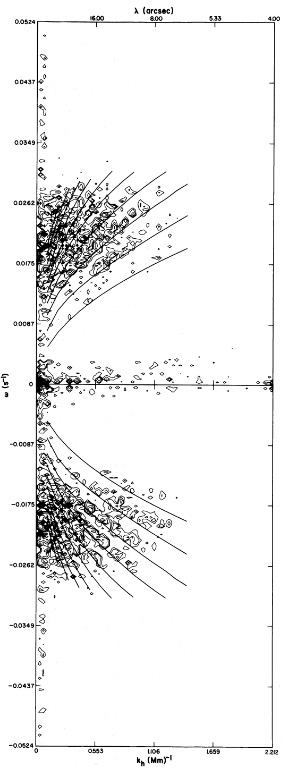
\includegraphics[keepaspectratio,angle=0,width=0.75\textwidth]{rotationshiftridge}
\end{figure}

\end{column}

\end{columns}

\end{frame}

\begin{frame}{Splitting delle frequenze per campo velocit\'a rotazionale}

L'equazione del moto al primo ordine nella perturbazione, con $\alpha=(l,m)$, \'e:
\begin{equation}\label{eq:eomrotation}
\begin{split}
&\rho_0(\omega_{\alpha}^2+2\omega_{\alpha}\Delta\omega_{\alpha})\vec{\xi}=\\
&\nabla P_1-\frac{\rho_1}{\rho_0}\nabla P_0+\rho_0\nabla\Phi_1+2i\omega_{\alpha}\rho_0(\scap{v_0}{\nabla})\vec{\xi}
\end{split}
\end{equation}
%dove ho esplicitato il termine inerziale \eqref{eq:inertialtermvf} e usando $(\scap{v_0}{\nabla})\vec{\xi}=im\vec{\Omega}\xi+\vecp{\Omega}{\xi}$, lo splitting dovuto alla rotazione \'e:
\begin{equation*}%\label{eq:splitfreqrotation}
\begin{split}
&\Delta\omega_{\alpha}=\frac{i\int\rho_0\xi_{\alpha}^*(\scap{v_0}{\nabla})\xi_{\alpha}\,d^3x}{\int\rho_0\xi_{\alpha}^*\xi_{\alpha}\,d^3x}\\
&=\frac{-m\int\rho_0\Omega\xi_{\alpha}^*\xi_{\alpha}\,d^3x+i\int\rho_0\xi_{\alpha}^*(\vecp{\Omega}{\xi_{\alpha}})\,d^3x}{\int\rho_0\xi_{\alpha}^*\xi_{\alpha}\,d^3x}
\end{split}
\end{equation*}

%La velocit\'a angolare contribuisce a $\Delta\omega_{\alpha}$ negli strati in cui $\xi_{\alpha}$ \'e apprezzabile.
\end{frame}

\begin{frame}{Espressioni semplificate}

%Nel caso di rotazione dipendente solo da r si ha che $\Delta\omega_{\alpha}$ \'e lineare in m: ho $2l+1$ frequenze equispaziate e 
Per modi p di alto n e $\Omega(r)$ approssimo lo splitting delle frequenze con:
\begin{align*}
&\delta\omega_{nlm}\approx m\frac{\int_{r_t}^R\Omega(r)\,\frac{dr}{c}}{\int_{r_t}^R\frac{dr}{c}}\\
%\intxt{per $\Omega(r)$ puramente radiale, cio\'e  per una media sulla latitudine; per velocit\'a angolare generale $\Omega(r,\theta)$, usando le propriet\'a dei polinomi di Legendre $P_l^m(x)$:}
&\delta\omega_{nlm}\approx m\frac{\int_{\cos{\Theta}}^{-\cos{\Theta}}(\cos^2{\Theta}-\cos^2{\theta})\expy{-\frac{1}{2}}\int_{r_t}^R(1-\frac{L^2c^2}{r^2\omega^2})\expy{\frac{1}{2}}\Omega(r,\theta)\frac{dr}{c}\,d(\cos{\theta})}{\int_{r_t}^R(1-\frac{L^2c^2}{r^2\omega^2})\expy{\frac{1}{2}}\,\frac{dr}{c}}
%&\Theta=\sin^{-1}{(\frac{m}{L}).}
\end{align*}

Le autofunzioni hanno ampiezza apprezzabile nella fascia compresa tra le latitudini $\pm\Theta=\pm \sin^{-1}{(\frac{m}{L})}$.

%Il problema di trovare $\Omega(r,\theta)$ dalla differenza $\Delta\omega_{\alpha}$ \'e lineare in $\Omega$ quindi $\Delta\omega_{\alpha}\propto\Omega$. Per determinare quindi la rotazione si utilizzano tecniche di inverzione basate sul principio variazionale.

%Parametrizzano le frequenze nel multipletto $(n,l)$ tramite:
\begin{equation}
\nu_{nlm}=\nu_{nl0}+\sum_{j=1}^{j_{\max}}a_j(n,l)\pol_j^{(l)}(m)\label{eq:freqmulti}
\end{equation}
%e ricavo i coefficienti tramite fit con le frequenze osservate; i 
Coefficienti dispari: il contributo della rotazione al termine lineare.

Coefficienti pari: effetti delle asfericit\'a nella struttura solare e effetti quadratici della rotazione.

\end{frame}

\section{Caratteristiche asintotiche delle oscillazioni adiabatiche}


\subsection{Comportamento asintotico dei modi.}

\begin{frame}{Approssimazione di Cowling}

(\cite{cow41oscillations})
\begin{equation}
\Phi'(r)=-\frac{4\pi G}{2l+1}\left[\frac{1}{r^{l+1}}\int_0^r\rho'(r)r'^{l+2}\,dr'+r^l\int_r^R\frac{\rho'(r')}{r'^{r'^{l-1}}}\,dr'\right]\label{eq:perturbedgravitational}
\end{equation}

da cui si vede che $|\Phi'|$ \'e trascurabile rispetto a $\rho'$ sia nel caso in cui $l\gg1$, per l'esponente crescente con l al denominatore dei due addendi in \eqref{eq:perturbedgravitational}, sia nel caso $|n|\gg1$, per il comportamento rapidamente oscillante di $\rho'$.

Il sistema \eqref{eigenomega} si riduce a:
\begin{subequations}\label{cowosc:main}
\begin{align}
&\frac{1}{r^2}\TDof{r}(r^2\xi_r)-\frac{\xi_rg_0}{c^2}+\frac{1}{\rho_0}(\frac{1}{c^2}-\frac{l(l+1)}{r^2\omega^2})P'=0\label{cowosc:a}\\
&\frac{1}{\rho_0}(\TDof{r}+\frac{g}{c^2})P'-(\omega^2-N^2)\xi_r=0\label{cowosc:b}
\end{align}
\end{subequations}

\end{frame}

\subsection{Relazione di dispersione per i modi gravo-acustici.}

\begin{frame}{Relazione di dispersione approssimata}

\begin{block}{Approssimazione di onda piana}
%Approssimo il comportamento spaziale delle oscillazioni localmente con un'onda piana $\vec{\xi}\propto\exp{i\scap{k}{x}}$ con $\vec{k}=k_r\hat{r}+\vec{k}_h$.
%\'E utile fare l'ulteriore approssimazione, valida per grandi n, di trascurare la variabile perturbata rispetto alla sua derivata radiale, e cos\'i si ottiene
\begin{equation}\label{eq:secondorder}
\TtwoDy{r}{\xi_r}=\frac{\omega^2}{c_s^2}(1-\frac{N^2}{\omega^2})(\frac{S_l^2}{\omega^2}-1)\xi_r=-K(r)\xi_r
\end{equation}
%$K(r)>0$: comportamento oscillante con
%\begin{equation}
%K(r)=k_r^2=\frac{\omega^2}{c_s^2}(\frac{N^2}{\omega^2}-1)(\frac{S_l^2}{\omega^2}-1)\label{eq:approximatedispersion}
%\end{equation}
%Le approssimazioni fatte non sono pi\'u valide vicino alla superficie dove il termine in $\invers{H_P}$ non \'e trascurabile per $H_P$ piccolo e vicino al centro solare dove il termine in $\frac{2}{r}$ non \'e trascurabile.

\end{block}

\begin{block}{Frequenza acustica critica}

Considero \eqref{cowosc:main}  per lunghezza d'onda delle perturbazioni molto minore della scala caratteristica di variazione di $N, c$.
\begin{align*}
%&\xi_r\propto\rho_0\expy{-\frac{1}{2}}\exp{ik_rr},\ P_1\propto\rho_0\expy{\frac{1}{2}}\exp{ik_rr}\\
%\intxt{dove la dipendenza dalla densit\'a di equilibrio \'e dovuta alla conservazione dell'energia. Definisco la frequenza critica acustica:}
&\omega_A=\frac{c_s}{2\densityscale{}}\sqrt{1-2\TDy{r}{\densityscale{}}}\propto T\expy{-\frac{1}{2}}\\%\label{eq:acusticcutoff}\\
%\intxt{quindi ottengo la relazione di dispersione:}
&k_r^2=\frac{\omega^2-\omega_A^2}{c^2}+S_l\frac{N^2-\omega^2}{c^2\omega^2}=\frac{\omega^2}{c^2}(1-\frac{\omega_{l,+}^2}{\omega^2})(1-\frac{\omega_{l,-}^2}{\omega^2})\\%\label{eq:localdispersion}\\
%\intxt{dove ho definito le frequenze critiche per i modi gravo-acustici}
&\omega_{\pm}=\frac{1}{2}(S_l^2+\omega_c^2)\pm\sqrt{\frac{1}{2}(S_l^2+\omega_c^2)^2-N^2S_l^2}
\end{align*}

\end{block}

\end{frame}

\subsection{Cavit\'a risonanti.} \label{sec:resonantcavity} %Definizione frequenze critiche

\begin{frame}{Frequenze critiche}

%\begin{minipage}{\linewidth}
\begin{tikzpicture}
\node[inner sep=0pt] (image) at (-0.5,0)
  {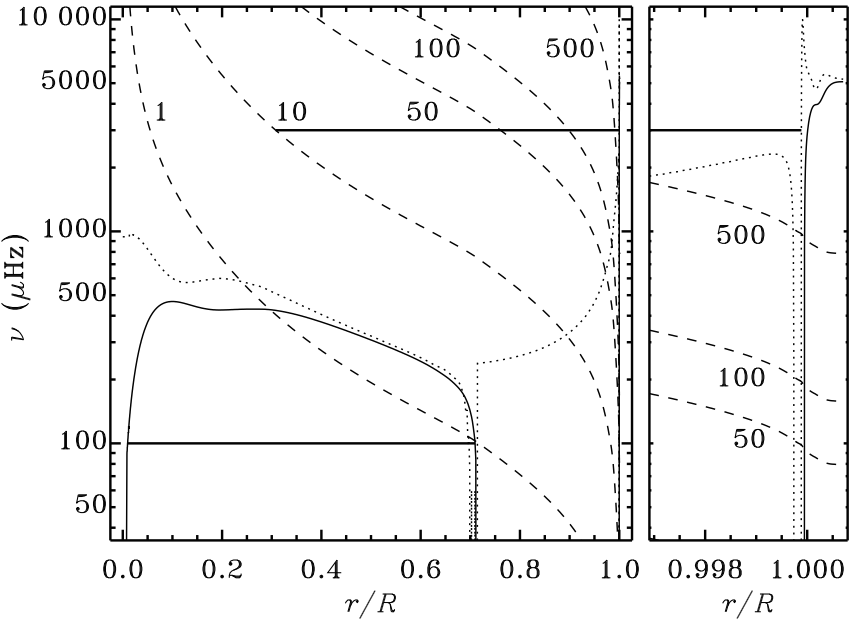
\includegraphics[keepaspectratio=true,width=0.5\textwidth]{cutoff}};
  \node (legenda) at (5.8,3) { Legenda };
  %\draw [draw=black!50] (legenda.north west) rectangle +(0.35\textwidth, -4cm);
  \draw [dotted] (6,2) -- (5.5,2) node[at start, anchor=west] {$\frac{\omega_c}{2\pi}$;};
  \draw [dashed] (7.5,2) -- (7,2) node[at start, anchor=west] {$\frac{S_l}{2\pi}$;};
  \draw [] (9,2) -- (8.5,2) node[at start, anchor=west] {$\frac{N}{2\pi}$;};
  %\node at (7.9,0.5) {\parbox{0.32\textwidth}{Le linee orizzontali a \SI{100}{\micro\hertz} e \SI{3000}{\micro\hertz} demarcano le regione in cui sono confinati risp. un modo g e p.}};
  %\node (caption) at (7.6,-2.3) { \begin{minipage}[l]{0.4\textwidth}
%\captionof{figure}{Frequenze caratteristiche calcolate tramite il modello S. Da \cite{chr02helioseismology}.\label{cutoff}}%   
    %\end{minipage}};
\end{tikzpicture}
%\end{minipage}

\end{frame}

\begin{frame}{Cavit\'a risonanti}

Le onde acustiche sono confinate in una regione che \'e limitata superiormente dall'aumento della frequenza critica acustica
\begin{equation}
\omega_A=\frac{c_s}{2\densityscale{}}\sqrt{1-2\TDy{r}{\densityscale{}}}\propto T\expy{-\frac{1}{2}}\label{eq:acusticcutoff}
\end{equation}
%causato dalla diminuzione della temperatura che provoca la riflessione delle onde con periodo attorno ai 5-min, mentre l'aumento della velocit\'a del suono con la profondit\'a e la conseguente rifrazione dell'onda porta a propagazione del moto puramente tangenziale
e inferiormente dall'aumento di $c_s$ per cui $k_r=0$ nel guscio sferico dove $c_s=\frac{\omega}{k_h}\approx\omega \frac{r}{L}$ ovvero per $\omega=S_l$ frequenza di Lamb definita da
\begin{equation}
S_l^2=\frac{l(l+1)c_s^2}{r^2}\label{eq:Lambf}
\end{equation}
In termini del raggio di inversione del moto:
\begin{equation}
\frac{c(r_t)}{r_t}=\frac{\omega}{L}
\end{equation}

Le regione di propagazione dei modi g sono definite da $\omega<N$: i modi g sono confinati nelle regioni pi\'u interne del Sole.
%Le onde di gravit\'a sono presenti nelle regioni in cui il gas \'e neutro o completamente ionizzato ($N^2$ grande) mentre sono riflesse dalle regioni dove $N$ \'e piccolo o immaginario: ionizzazione parziale, instabilit\'a convettiva, centro del Sole.
I modi g sono confinati tra la la parte centrale dove $g\to0$ e il fondo della zona convettiva dove $N^2<0$.

\end{frame}

\begin{frame}{Traiettoria delle onde}

\begin{figure}[!ht]
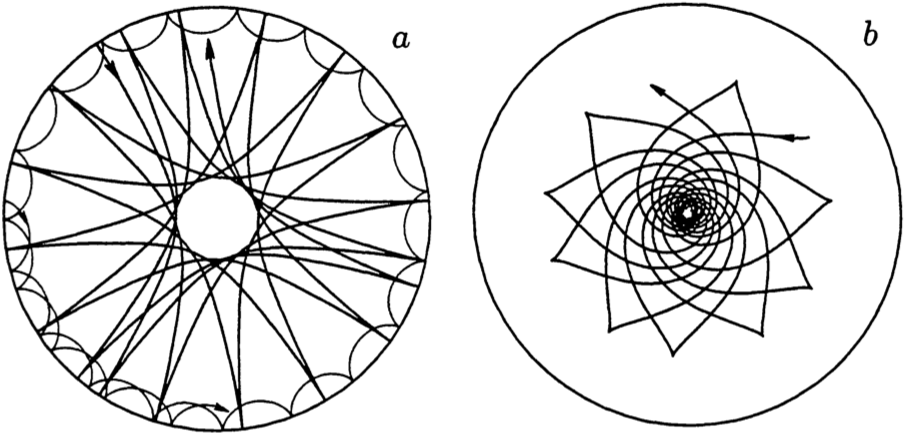
\includegraphics[keepaspectratio,width=0.8\textwidth]{raypath-gp}
\caption{(a): Percorso di due onda acustiche $p_8(l=2), p_8(l=100)$; (b): Percorso di un'onda di gravit\'a: $g_{10}(l=5)$. Da\cite{gou91seismic}.}
\end{figure}

\end{frame}

\begin{frame}{Raggio di inversione del moto}

\begin{figure}[!ht]
\centering
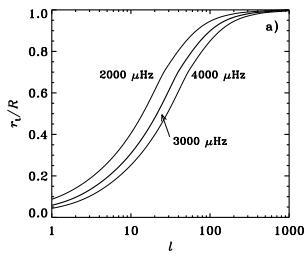
\includegraphics[keepaspectratio,angle=0,width=0.6\textwidth]{plowertp}
\caption{Andamento del raggio di inversione del moto in funzione del grado l. Da \cite{dal03notes}.}\label{fig:plowertp}
\end{figure}

\end{frame}

\subsection{Condizione di risonanza radiale}

\begin{frame}{Legge di Duvall}

\begin{minipage}{0.55\textwidth}

\begin{figure}[!ht]
\centering
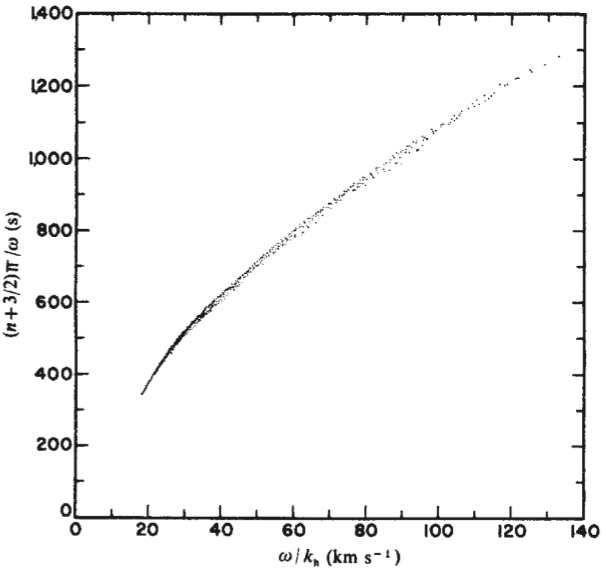
\includegraphics[keepaspectratio,width=0.99\textwidth]{dispersionDuvall}
\end{figure}

\end{minipage}
\begin{minipage}{0.4\textwidth}

\captionof{figure}{I modi p sono allineati su un'unica curva, dove n \'e l'ordine radiale e $\alpha$ una fase dovuta alla riflessione. Da \cite{duv82dispersion}.}\label{fig:duv82dispersion}

\end{minipage}

%Questo comportamento \'e stato osservato per i modi p da \citet{duv82dispersion}. Un grafico di $\frac{\pi(n+\alpha)}{\omega}$ rispetto a $\frac{\omega}{k_h}$ rappresenta i modi p con un'unica curva (vedi \ref{fig:duv82dispersion}), per $\alpha$ opportuno con:
%\begin{equation}
%(n+\alpha)\frac{\pi}{\omega}=F'(\frac{\omega}{k_h})=F(\frac{\omega}{L})\label{eq:duvallr}
%\end{equation}
%e usando la relazione di dispersione per onde acustiche \eqref{eq:approximatedispersion}
%\begin{equation}
%k_r^2\frac{\omega^2}{c_s^2}(\frac{S_l^2}{\omega^2}-1)
%\end{equation}
%si ha:
\begin{align}
&F(w)=\int_{r_t}^R\sqrt{1-\frac{c_s^2}{r^2w^2}}\,\frac{dr}{c_s}\label{eq:duvallf}\\
&(n+\alpha)\pi\approx\int_{r_t}^Rk_r\,dr\approx\int_{r_t}^R\frac{\omega}{c_s}\sqrt{1-\frac{S_l^2}{\omega^2}}\,dr\label{eq:duvallexpli}
\end{align}

\end{frame}

\begin{frame}{Condizione di risonanza radiale}

Le frequenze dei modi sono determinate dalla condizione, per l fissato, che l'onda interferisca costruttivamente con se stessa. Un'onda stazionaria in direzione radiale implica che l'integrale di $k_r$ nella regione di propagazione fra due zeri consecutivi sia un intero multiplo di $\pi$:
\begin{equation}
\omega\int_{r_1}^{r_2}\sqrt{1-\frac{\omega_A^2}{\omega^2}-\frac{S_l^2}{\omega^2}(1-\frac{N^2}{\omega^2})}\,\frac{dr}{c}\approx\pi(n-\frac{1}{2})\label{eq:JWKBmode}
\end{equation}
che tiene conto del numero dei nodi radiali e dello sfasamento $\alpha$ prodotto nelle regioni di riflessione.


%$Utilizzando invece il limite per basse frequenze di \eqref{eq:approximatedispersion} per i modi g trovo la relazione di dispersione approssimata per $l\neq0$:
%\begin{equation}
%k_r^2=\frac{S_l^2}{c^2}(\frac{N^2}{\omega^2}-1)\label{eq:dispersionag}
%\end{equation}
%[introdotta in precedenza \eqref{eq:bvf}]

Espressione analoga di \eqref{eq:duvallexpli} per i modi g:
\begin{equation}\label{eq:duvallg}
\frac{(n+\alpha_g)\pi}{L}\approx\int_{r_1}^{r_2}(\frac{N^2}{\omega^2}-1)\expy{\frac{1}{2}}\,d\ln{r}
\end{equation}
con $r_2\approx R_{cz}$ e $\alpha_g$ \'e una fase dovuta alla riflessione e dipende dall'andamento di $N^2$ nella regione di inversione del moto, alla base della zona convettiva.

\end{frame}

\subsection{Espressioni asintotiche delle frequenze dei modi}

\begin{frame}{Espressioni asintotiche}

%\begin{block}{Modi p confinati nella zona convettiva}
%Per modi di alto grado angolare, confinati nella regione convettiva, considerando $\Gamma_1$ e $g$ lentamenta variabili e una stratificazione adiabatica, 
%Considero stratificazione adiabatica:
%\begin{equation}
%\omega^2=\frac{2}{\mu_p}\frac{g}{R}(n+\alpha)
%\end{equation}
%dove $\mu_p=\frac{1}{\Gamma_1-1}$ \'e l'inidce politropico efficace .
%\end{block}

\begin{columns}

\begin{column}{0.5\textwidth}

\begin{block}{Modi p di basso l}
%I modi di basso l penetrano in profondit\'a, quindi approssimo $r_t\approx0$, e, usando l'espansione
%\begin{equation}
%F(w)\approx\int_0^R\frac{dr}{c}-w\expy{-1}\frac{\pi}{2}\label{eq:Flinear}
%\end{equation}
% risulta
%\begin{equation}
%\int_0^R\frac{dr}{c}-\frac{L}{\omega}\frac{\pi}{2}=\frac{(n+\alpha)\pi}{\omega}
%\end{equation}
Frequenze sono equispaziate in n e $\nu_{nl}\approx\nu_{n-1,l+2}$:

\begin{equation}
\frac{\omega_{nl}}{2\pi}\approx(n+\frac{l}{2}+\frac{1}{4}+\alpha)\Delta\nu\label{eq:freqequi}
\end{equation}
con $\Delta\nu=[2\int_0^R\frac{dr}{c}]\expy{-1}\approx\SI{136}{\micro\hertz}$.

\end{block}

\end{column}

\begin{column}{0.5\textwidth}

\begin{block}{Modi g di basso l}

%Per i modi g approssimo \eqref{eq:JWKBmode} con
%\begin{equation}
%\int_{r_1}^{r_2}\sqrt{\frac{N^2}{\omega}-1}\frac{dr}{r}=\frac{(n-\frac{1}{2})\pi}{L}
%\end{equation}
%dove l'integrale comprende la regione di propagazione e i punti di inversione del moto sono definiti dall'andamento di N.

I modi g di alto n e basso l soddisfano un'equazione analoga a \eqref{eq:freqequi} con periodi equispaziati
\begin{equation}
\omega=\frac{L\int_{r_1}^{r_2}N\frac{dr}{r}}{\pi(n+\frac{l}{2}+\alpha_g)}
\end{equation}
e $\lim_{n\to\infty}{\alpha_g}\approx-\midfrac{1}{6}$.

\end{block}

\end{column}

\end{columns}

\end{frame}